\documentclass[a4paper,journal]{IEEEtran}
\usepackage{amsmath,amsfonts}
\usepackage{algorithmic}
\usepackage{array}
\usepackage{cite}
\usepackage[caption=false,font=normalsize,labelfont=sf,textfont=sf]{subfig}
\usepackage{textcomp}
\usepackage{stfloats}
\usepackage{url}
\usepackage{verbatim}
\usepackage[english,spanish,mexico]{babel}
\usepackage{blindtext}
\usepackage[utf8]{inputenc}
\usepackage{graphicx}
\usepackage{balance}
\begin{document}
\title{Bolómetro: Principios de Funcionamiento.\\}
\author{Alexis L. Ayala, Leonardo G. Vazquez\\Escuela Superior de Ingeniería Mecánica y Eléctrica Unidad Zacatenco\\ Detección Óptica\\Profesor: Dr. Eduardo M. Casas\\ aayalal1600@alumno.ipn.mx ,lgutierrezv1701@alumno.ipn.mx}
\markboth{Ingenieria en Fotónica, Archivo No.~1 15 de Abril del 2024}{15 de Abril del 2024}
\maketitle
%Resumen y abstract
\selectlanguage{spanish}
\begin{abstract}
  En el presente trabajo se revisarán los principios físicos que rigen el funcionamiento de un bolómetro, un dispositivo sensible al calor (radiación infrarroja). Se proporcionará una introducción a las teorías elementales de respuesta del bolómetro, de la radiación térmica y del ruido propio del dispositivo, así como una descripción de las partes que lo constituyen y la tarea a realizar por cada una de ellas. Se indica cómo su perfil coincide con la clase más común de detectores térmicos y se describen las aplicaciones para las cuales la solución es óptima. También se analizarán las teorías más rigurosas de respuesta y ruido necesarias para una mejor comprensión del tema.\\ 
  Se hablará sobre la radiación infrarroja en general, los detectores de radiación infrarroja, la estructura de un bolómetro, los tipos de bolómetros y las aplicaciones de interés. \\
  En resumen, en este artículo se ofrece una visión de la tecnología bolométrica, desde sus fundamentos teóricos básicos hasta su aplicación práctica en diversas condiciones, destacando su importancia en la detección y medición de radiación infrarroja y milimétrica en varios campos científicos, tecnológicos e industriales. 
\end{abstract}
%%Palabras clave
\begin{quote}
        \bf
        \small
        \emph{Palabras Clave}—Principios físicos, calor, radiación infrarroja, teorías elementales, respuesta, radiación térmica, ruido, detectores térmicos, detectores, estructura, aplicaciones, tecnología bolométrica, fundamentos teóricos, detección, medición, milimétrica, campos científicos. 
\end{quote}

\selectlanguage{english}
%Abstract
\begin{abstract}
This paper will review the physical principles governing the operation of a bolometer, a device sensitive to heat (infrared radiation). An introduction to the elementary theories of bolometer response, thermal radiation and device self-noise will be provided, as well as a description of its constituent parts and the task to be performed by each of them. It is indicated how its profile matches the most common class of thermal detectors and the applications for which the solution is optimal are described. The more rigorous theories of response and noise necessary for a better understanding of the subject will also be discussed. 
\\We will discuss infrared radiation in general, infrared radiation detectors, the structure of a bolometer, types of bolometers, and applications of interest. 
\\
In summary, this article provides an overview of bolometer technology, from its basic theoretical foundations to its practical application in various conditions, highlighting its importance in the detection and measurement of infrared and millimeter radiation in various scientific, technological and industrial fields. 
\end{abstract}
%%Keywords
\begin{IEEEkeywords}
Physical principles, heat, infrared radiation, elementary theories, response, thermal radiation, noise, thermal detectors, detectors, structure, applications, bolometric technology, theoretical foundations, detection, measurement, millimeter, scientific fields.
\end{IEEEkeywords}
%%Introducción
\selectlanguage{spanish}
\vspace{0.5cm}
\section{Introducción}
\IEEEPARstart{L}{a} radiación infrarroja es una clasificación de los distintos tipos de energía electromagnética, estas se clasifican según su longitud de onda, frecuencia o energía. Este tipo de radiación electromagnética cuya longitud onda es mayor que la luz visible roja y menor que las microondas (Vease la figura 1).\\
Se encuentra por tanto fuera del espectro de ondas visibles por el ojo humano. La radiación infrarroja se denomina también radiación térmica ( calor radiante), y es emitida por todos los objetos calientes como motores calientes, metales en fusión y otras fuentes de calor en fundiciones, lampara eléctricas incandescentes, sistemas de calefacción radiante, etc.
\begin{figure}[h]
\centering
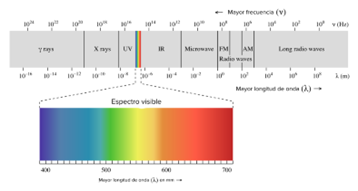
\includegraphics[width=2.5in]{spectre}
\caption{Espectro de radiación electromagnético.}
\label{spectre}
\end{figure}
\\ 
Todo objeto por encima de 0°k emite radiación infrarroja y se produce por el calor de dicho cuerpo, por lo que el ser humano se encuentra expuesto en pequeñas cantidades al realizar diversas ocupaciones de la vida cotidiana, por ejemplo, en el hogar o durante las actividades recreativas realizadas al sol. Por lo que es importante el estudio y elaboración de detectores de radiación infrarroja para el estudio de los fenómenos relacionados con esta en diversas áreas, desde la investigación científica, aplicaciones médicas, seguridad y vigilancia, industrial y control de calidad, hasta las aplicaciones cotidianas.
\\
Una forma de detectar la radiación infrarroja incidente es mediante un dispositivo llamado bolómetro. Esta palabra proviene de griego “bole” lo cual significa rayo de luz y “metrón”, medida. El astrónomo Samuel Pierpont Langley lo inventó en 1878.
\\

%%Principio de Funcionamiento de un Bolometro
\section{Principio de funcionamiento de un Bolómetro}
Hoy en día los detectores infrarrojos se dividen en dos grandes grupos.
\begin{itemize}
  \item El primer grupo se conoce como detectores de efecto cuántico, se basa en la liberación de electrones en estructura en forma de rejilla. 
  \item El segundo grupo denominado detectores térmicos responde al calor emitido por los cuerpos cuando son expuestos a radiación. 
\end{itemize}
Los detectores de efecto cuántico son dispositivos que utilizan principios de la mecánica cuántica para detectar y medir la luz u otras formas de radiación electromagnética. \\
A diferencia de los detectores clásicos, que funcionan según el principio de que la energía de la luz es absorbida por un material y luego convertida en una señal eléctrica, los detectores de efecto cuántico pueden detectar fotones individuales, las partículas individuales de luz. 
\\Esto les permite lograr una mayor sensibilidad y precisión que los detectores clásicos.
\\
Los detectores de efecto térmico, también conocidos como detectores térmicos, son dispositivos que detectan cambios en la temperatura midiendo la radiación infrarroja (IR) emitida por un objeto. 
\\A diferencia de los detectores de humo tradicionales, que detectan partículas de humo en el aire, los detectores de efecto térmico no necesitan que el humo esté presente para activarse. Esto los hace más efectivos para detectar incendios que se desarrollan lentamente o que producen poco humo.

%%Empieza el principio de funcionamiento de un bolometro
\subsection[Principio de funcionamiento de un bolómetro]{Principio de funcionamiento de un bolómetro}
Un bolómetro funciona a partir de la conversión de la energía radiante (luz) en calor, que se mide para determinar la potencia de la radiación original.\\
Un bolómetro en sí no mide directamente en ninguna unidad estándar estos miden un cambio de temperatura debido a la radiación absorbida. Este cambio de temperatura suele medirse en grados Celsius (Kelvin).\\
Sin embargo, la finalidad última del bolómetro es determinar la potencia de la radiación incidente. Conociendo la relación entre el cambio de temperatura medido y la potencia de radiación absorbida (a través de la calibración y las propiedades del material), el bolómetro puede utilizarse para medir indirectamente la potencia. Para este fin, la unidad estándar para la potencia de radiación serían los volts (W) o sus derivados como los milivolts (mW) o los microvolts (µW).\\
%%Termina Principio de Funcionamiento de un Bolometro
\end{document}
